\documentclass{article}

\usepackage[utf8]{inputenc}
\usepackage[russian]{babel}
\usepackage[a4paper, margin=1in]{geometry}
\usepackage{graphicx}
\usepackage{amsmath}
\usepackage{wrapfig}
\usepackage{multirow}
\usepackage{mathtools}
\usepackage{pgfplots}
\usepackage{pgfplotstable}
\usepackage{setspace}
\usepackage{changepage}
\usepackage{caption}
\usepackage{csquotes}
\usepackage{hyperref}
\usepackage{listings}

\pgfplotsset{compat=1.18}
\hypersetup{
  colorlinks = true,
  linkcolor  = blue,
  filecolor  = magenta,      
  urlcolor   = darkgray,
  pdftitle   = {
    database-report-1-smirnov-victor-p33131
  },
}

\definecolor{codegreen}{rgb}{0,0.6,0}
\definecolor{codegray}{rgb}{0.5,0.5,0.5}
\definecolor{codepurple}{rgb}{0.58,0,0.82}
\definecolor{backcolour}{rgb}{0.99,0.99,0.99}

\lstdefinestyle{codestyle}{
  backgroundcolor=\color{backcolour},   
  commentstyle=\color{codegreen},
  keywordstyle=\color{magenta},
  numberstyle=\tiny\color{codegray},
  stringstyle=\color{codepurple},
  basicstyle=\ttfamily\footnotesize,
  breakatwhitespace=false,         
  breaklines=true,                 
  captionpos=b,                    
  keepspaces=true,                 
  numbers=left,                    
  numbersep=5pt,                  
  showspaces=false,                
  showstringspaces=false,
  showtabs=false,                  
  tabsize=2
}

\graphicspath{ {./img/} }

\lstset{style=codestyle}

\begin{document}

\begin{titlepage}
    \begin{center}
        \begin{spacing}{1.4}
            \large{Университет ИТМО} \\
            \large{Факультет программной инженерии и компьютерной техники} \\
        \end{spacing}
        \vfill
        \textbf{
            \huge{Базы данных.} \\
            \huge{Лабораторная работа №1.} \\
        }
    \end{center}
    \vfill
    \begin{center}
        \begin{tabular}{r l}
            Группа:  & P33131                  \\
            Студент: & Смирнов Виктор Игоревич \\
            Вариант: & 310963
        \end{tabular}
    \end{center}
    \vfill
    \begin{center}
        \begin{large}
            2023
        \end{large}
    \end{center}
\end{titlepage}

\section*{Ключевые слова}

База данных, PostgreSQL,
даталогическая модель,
инфологическая модель.

\tableofcontents

\section{Цель работы}

Научиться проектировать базы данных,
составлять инфологические и
даталогические модели данных,
реализовывать их в БД
PostgreSQL, научиться выполнять
запросы.

\section{Текст задания}

Как бы там ни было, вид спускающихся с дерева
загадочных существ произвел слишком тягостное
впечатление на динозавриху. Загоготав на
прощание, животное подтолкнуло малыша и
медленно поплелось прочь.

\section{Описание предметной области}

Из текста сразу выделяем действующие лица:
загадочное существо, динозавриха,
малыш -- их можно назвать одним словом --
существа. У существ есть имя, пол, они что-то
чувствуют, что-то делают и где-то находятся.
Чувств, действий и местоположений может быть
немеренное количество, поэтому их целесообразно
выделить в отдельные таблицы для гибкости схемы
данных.

\section{Классификация сущностей}

\begin{enumerate}
    \item \texttt{creature} -- стержневая сущность
    \item \texttt{kind} -- характеристическая сущность
    \item \texttt{location} -- характеристическая сущность
    \item \texttt{emotion} -- характеристическая сущность
    \item \texttt{action} -- характеристическая сущность
\end{enumerate}

\section{Инфологическая модель}

\begin{figure}[th]
    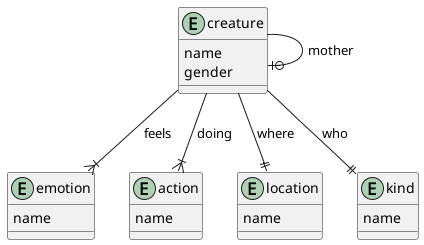
\includegraphics[scale=0.5]{./high-er-diagram.png}
    \centering
\end{figure}

\newpage

\section{Даталогическая модель}

\begin{figure}[th]
    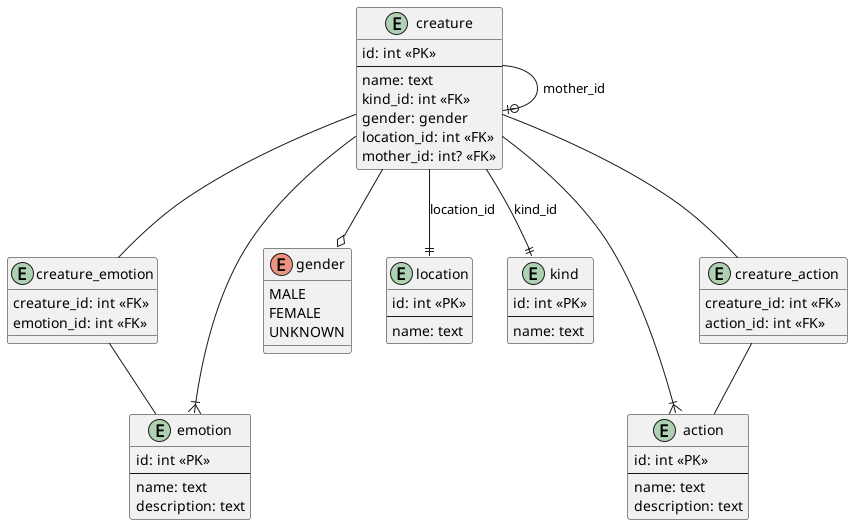
\includegraphics[scale=0.5]{./low-er-diagram.png}
    \centering
\end{figure}

\section{Реализация на PostgreSQL}

\lstinputlisting[language=SQL]{../../../src/scheme/01-init-tables.sql}

\section{Вывод}

Проектирование БД -- непростое занятие, которое
лучше осуществлять итеративно. Cначала
описать предметную область словами, чтобы лучше
понять суть проблемы. Далее опуститься на уровень
ниже и составить инфологическую модель данных,
которая никак не связана с конкретной БД, а
лишь выражает главные связи ваших данных.
Когда инфологическая модель будет готова,
по ней можно будет составить даталогическую
модель данных -- наиболее близкое к выбранной
БД представление. И только после выполения всех
вышеперечисленных шагов можно приступать
к реализации схемы БД на выбранном диалекте SQL,
так удасться свести риски неудачного дизайна БД
к минимуму.

\begin{thebibliography}{9}
    \item \href{https://www.postgresql.org}{
        PostgreSQL Home Page}

    \item \href{https://se.ifmo.ru/documents/10180/733702/isbd-2021-2.6.pdf/e47a2e01-d445-e017-070f-a300ecdb71a8}{
        ИТМО ВТ. Информационные системы и базы данных}

    \item \href{https://youtu.be/HnRXzrg3Sd4?si=Il3rxvHIpw93Wx0J}{
        Базы данных. Проектирование. R class Tech}
\end{thebibliography}

\end{document}